\section{Einleitung}

%----------------------------------------------------------------------%SLIDE -
\begin{frame}[c]
    \frametitle{Einleitung}
    \begin{columns}
        \column{0.5\textwidth}
        \begin{itemize}
            \item Moore's law
            \item Computer werden leistungsfähiger
            \item mehr Prozessoren machen ein Programm nicht schneller
            \item nicht von allein
        \end{itemize}
        \column{0.6\textwidth}
        \begin{figure}
            \centering
            \copyrightbox%
                {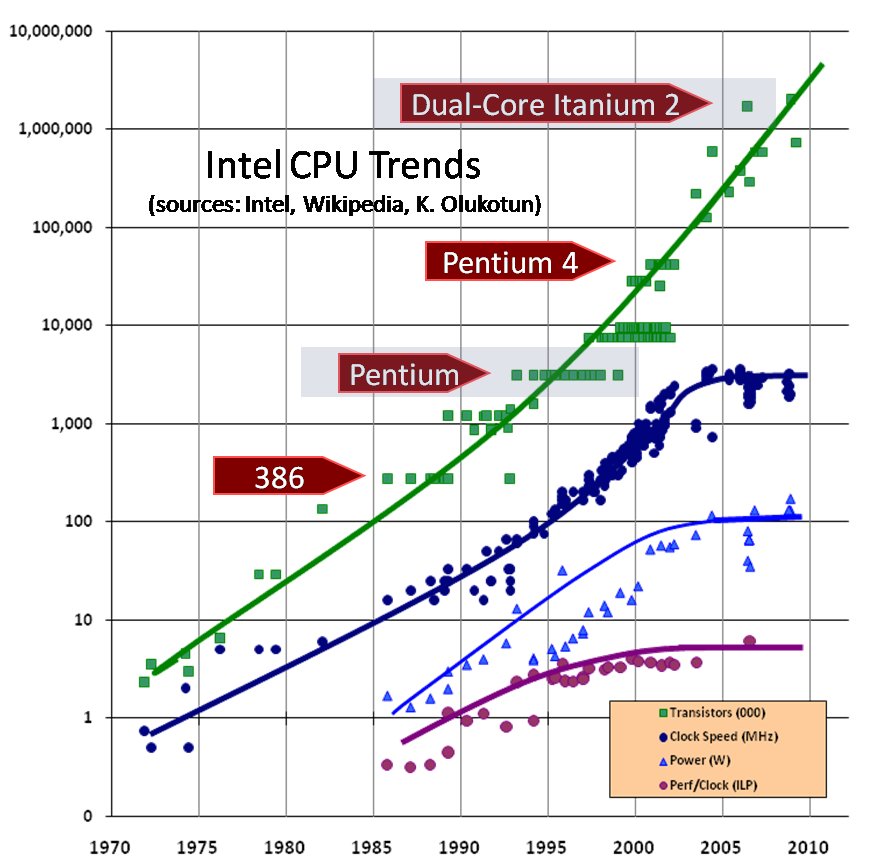
\includegraphics[height=0.6\textheight]{content/images/CPU}}%
                {by Herb Sutter \url{http://www.gotw.ca/publications/concurrency-ddj.htm}}
            \caption{Intel CPUs}
        \end{figure}
    \end{columns}
\end{frame}
%----------------------------------------------------------------------%SLIDE -
